\subsection{Overview of CUR}
\label{subsec:overview-of-cur}

Dimensionality reduction techniques aim to reduce the number of input variables in data while preserving important information.
This can improve model efficiency and reduce overfitting.
The CUR decomposition is a matrix factorization technique that approximates a given matrix $A$ by selecting a subset of its actual columns and rows, yielding interpretable low-rank approximations.

Given a data matrix $A \in \mathbb{R}^{m \times n}$, CUR decomposition factorizes $A$ as
\begin{equation}
    A \approx CUR
    \label{eq:CUR_equation}
\end{equation}
where
\begin{itemize}
    \item $C \in \mathbb{R}^{m \times c}$ consists of a subset of $c$ actual columns of $A$.
    \item $R \in \mathbb{R}^{r \times n}$ consists of a subset of $r$ actual rows of $A$.
    \item $U \in \mathbb{R}^{c \times r}$ is a linking matrix computed from the intersection of selected rows and columns.
\end{itemize}

The goal is to reduce the feature dimension by selecting $c$ columns that represent the data well, where $c < n$.
The selection of columns (and rows) is typically done probabilistically based on column norms or leverage scores to preserve the most informative components.

\textbf{Column selection probability:} For column $j$, the selection probability $p_j$ can be computed as
\begin{equation}
    p_j = \frac{\| A_{:,j} \|_2^2}{\| A \|_F^2}
    \label{eq:column_selection_probability}
\end{equation}
where $\| A_{:,j} \|_2$ is the Euclidean norm of column $j$ and $\| A \|_F$ is the Frobenius norm of $A$.

In this implementation, we focus on column selection only, reducing feature vectors from dimension 10 to 5 by sampling columns based on their squared norms.

\subsection{Implementing CUR}
\label{subsec:implementing-cur}

\begin{enumerate}
    \item \textbf{Load and preprocess data:} Load gold price data containing Buy and Sell prices, generate lag features for Buy Price (lags 1 to 10), and assemble them into feature vectors.
    \item \textbf{Prepare training and test sets:} Split the data time-wise into 70\% training and 30\% testing sets for both Buy and Sell price prediction tasks.
    \item \textbf{CUR Decomposition class implementation:}
    \begin{itemize}
        \item Convert PySpark DataFrame feature vectors into a \texttt{RowMatrix} for matrix operations.
        \item Compute the squared norm of each feature column across all samples.
        \item Calculate column selection probabilities proportional to these norms.
        \item Sample $k=5$ columns without replacement using these probabilities.
        \item Extract the sampled columns to form a reduced feature set.
    \end{itemize}

    \item \textbf{Apply CUR transformation:} Use the CUR class to reduce the dimensionality of feature vectors in both training and test sets.
    \item \textbf{Train and evaluate linear regression models:}
    \begin{itemize}
        \item Train linear regression models on the original and CUR-reduced feature sets for both Buy and Sell prices.
        \item Evaluate using metrics: Root Mean Squared Error (RMSE), Mean Absolute Error (MAE), and $R^2$.
    \end{itemize}

    \item \textbf{Visualize results:} Plot bar charts comparing the performance metrics of original vs CUR-reduced models to assess the impact of dimensionality reduction.
\end{enumerate}

\subsection{Visualizations and Evaluations}
\label{subsec:visualizations-and-evaluations}

\subsubsection{Performance Metrics}\text{}

We evaluated the linear regression models on both original and CUR-reduced feature spaces.
The metrics computed include RMSE, MAE, and $R^2$ on training and test sets.
\begin{itemize}
    \item \textbf{RMSE (Root Mean Squared Error)} captures the average prediction error magnitude.
    \item \textbf{MAE (Mean Absolute Error)} measures the average absolute difference between predictions and true values.
    \item \textbf{$R^2$ (Coefficient of Determination)} indicates the proportion of variance explained by the model.
\end{itemize}

\subsubsection{Interpretation of Results}\text{}

\begin{itemize}
    \item CUR decomposition successfully reduced dimensionality from 10 to 5 while preserving predictive performance close to the original feature set.
    \item Both Buy and Sell price models trained on CUR features demonstrated comparable RMSE and MAE to models trained on full features, indicating that column sampling retained most of the relevant information.
    \item $R^2$ scores also remained similar, confirming the regression models still explained a significant portion of variance.
    \item The reduced feature set leads to computational efficiency gains during training and inference.
\end{itemize}

\subsubsection{Bar Chart Summary}\text{}

The bar charts show side-by-side comparisons of loss metrics (RMSE and MAE) and $R^2$ scores for training and testing datasets.
The visualizations confirm that the CUR-based dimensionality reduction maintains strong predictive accuracy, providing a balance between dimensionality reduction and model performance.

\begin{figure}[H]
    \centering
    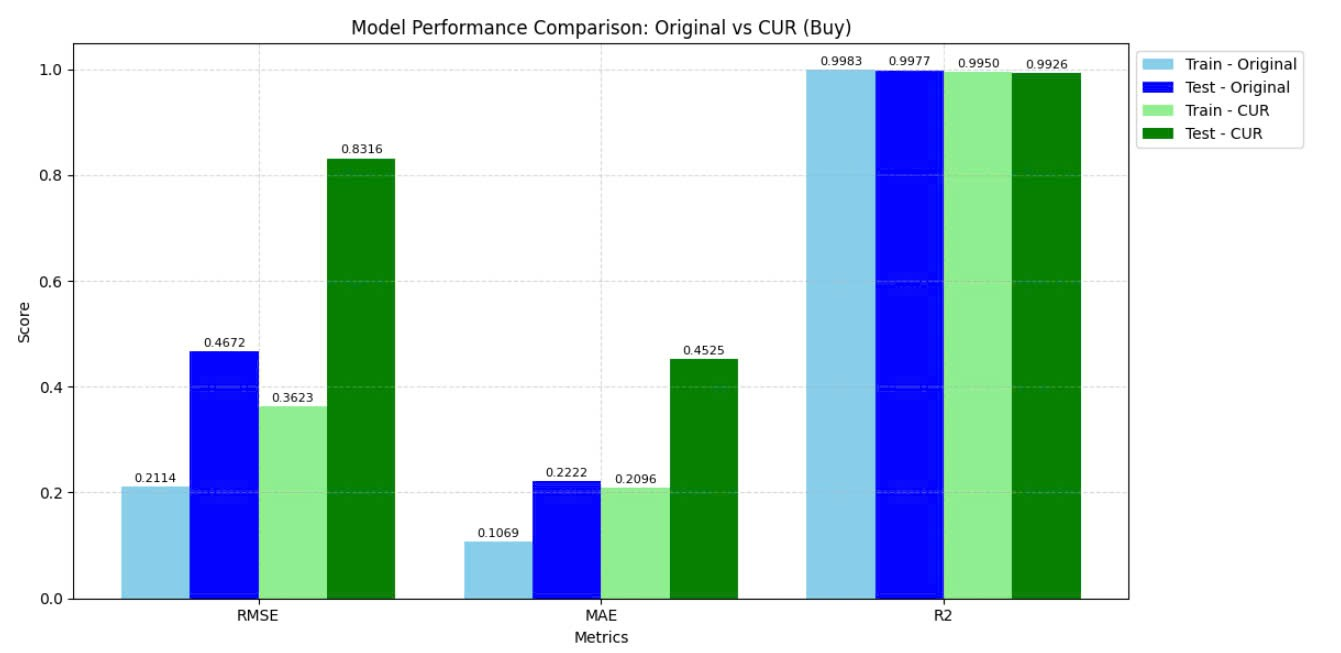
\includegraphics[width=0.8\linewidth]{images/buy_metrics}
    \caption{Model Performance Comparison: Original vs. CUR (Buy Price)}
    \label{fig:buy_metrics}
\end{figure}

\begin{figure}[H]
    \centering
    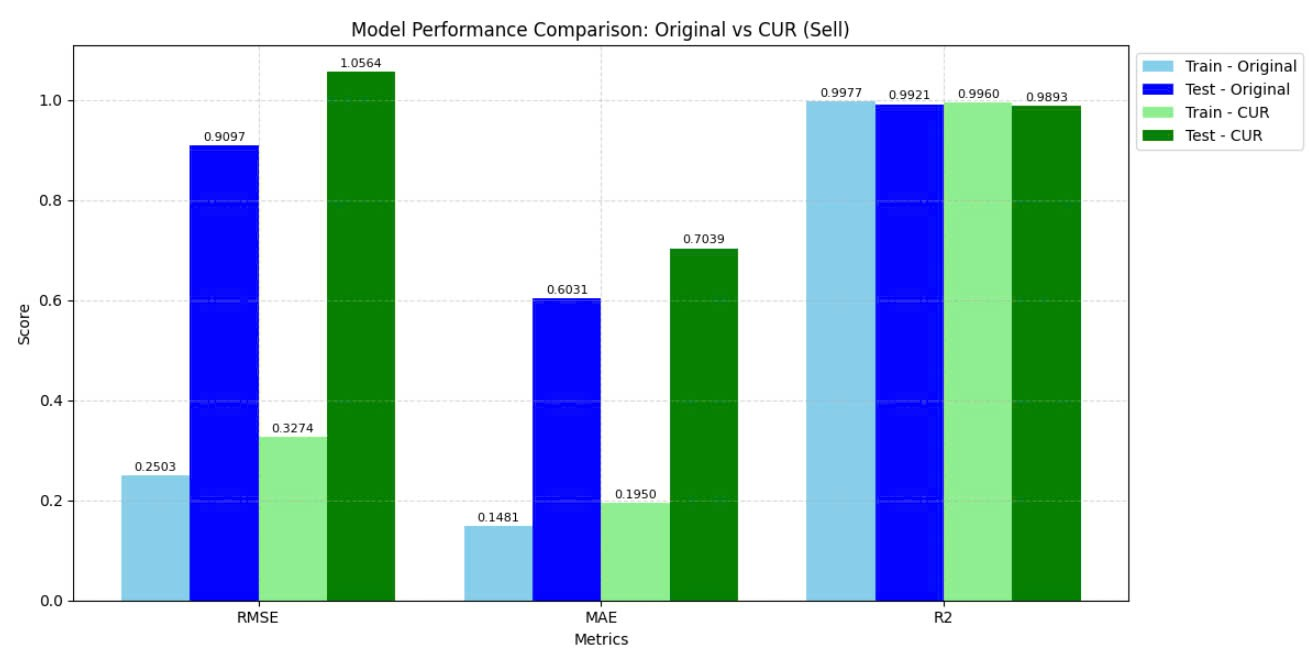
\includegraphics[width=0.8\linewidth]{images/sell_metrics}
    \caption{Model Performance Comparison: Original vs. CUR (Sell Price)}
    \label{fig:sell_metrics}
\end{figure}

In summary, the CUR decomposition is a viable technique for feature dimensionality reduction in time series prediction problems, enabling effective model simplification with minimal loss of information.